\documentclass[12pt,]{article}
\usepackage[]{times}
\usepackage{amssymb,amsmath}
\usepackage{ifxetex,ifluatex}
\usepackage{fixltx2e} % provides \textsubscript
\ifnum 0\ifxetex 1\fi\ifluatex 1\fi=0 % if pdftex
  \usepackage[T1]{fontenc}
  \usepackage[utf8]{inputenc}
\else % if luatex or xelatex
  \ifxetex
    \usepackage{mathspec}
  \else
    \usepackage{fontspec}
  \fi
  \defaultfontfeatures{Ligatures=TeX,Scale=MatchLowercase}
\fi
% use upquote if available, for straight quotes in verbatim environments
\IfFileExists{upquote.sty}{\usepackage{upquote}}{}
% use microtype if available
\IfFileExists{microtype.sty}{%
\usepackage{microtype}
\UseMicrotypeSet[protrusion]{basicmath} % disable protrusion for tt fonts
}{}
\usepackage[margin=1in]{geometry}
\usepackage{hyperref}
\hypersetup{unicode=true,
            pdftitle={Why Don't They Show Up?},
            pdfborder={0 0 0},
            breaklinks=true}
\urlstyle{same}  % don't use monospace font for urls
\usepackage{graphicx,grffile}
\makeatletter
\def\maxwidth{\ifdim\Gin@nat@width>\linewidth\linewidth\else\Gin@nat@width\fi}
\def\maxheight{\ifdim\Gin@nat@height>\textheight\textheight\else\Gin@nat@height\fi}
\makeatother
% Scale images if necessary, so that they will not overflow the page
% margins by default, and it is still possible to overwrite the defaults
% using explicit options in \includegraphics[width, height, ...]{}
\setkeys{Gin}{width=\maxwidth,height=\maxheight,keepaspectratio}
\IfFileExists{parskip.sty}{%
\usepackage{parskip}
}{% else
\setlength{\parindent}{0pt}
\setlength{\parskip}{6pt plus 2pt minus 1pt}
}
\setlength{\emergencystretch}{3em}  % prevent overfull lines
\providecommand{\tightlist}{%
  \setlength{\itemsep}{0pt}\setlength{\parskip}{0pt}}
\setcounter{secnumdepth}{0}
% Redefines (sub)paragraphs to behave more like sections
\ifx\paragraph\undefined\else
\let\oldparagraph\paragraph
\renewcommand{\paragraph}[1]{\oldparagraph{#1}\mbox{}}
\fi
\ifx\subparagraph\undefined\else
\let\oldsubparagraph\subparagraph
\renewcommand{\subparagraph}[1]{\oldsubparagraph{#1}\mbox{}}
\fi

%%% Use protect on footnotes to avoid problems with footnotes in titles
\let\rmarkdownfootnote\footnote%
\def\footnote{\protect\rmarkdownfootnote}

%%% Change title format to be more compact
\usepackage{titling}

% Create subtitle command for use in maketitle
\newcommand{\subtitle}[1]{
  \posttitle{
    \begin{center}\large#1\end{center}
    }
}

\setlength{\droptitle}{-2em}

  \title{Why Don't They Show Up?}
    \pretitle{\vspace{\droptitle}\centering\huge}
  \posttitle{\par}
    \author{}
    \preauthor{}\postauthor{}
    \date{}
    \predate{}\postdate{}
  
\usepackage[nofiglist, nofighead]{endfloat}
\usepackage[singlespacing]{setspace}
\usepackage{sectsty} \sectionfont{\centering}

\begin{document}
\maketitle

\section{ABSTRACT}\label{abstract}

Massive Open Online Courses (MOOCs) have gained prominence and
exponential growth over the last five years. Despite the high number of
registered participants, MOOCs are plagued by a high rate of
non-completion. In this study, we focus on crytallizing features that
are predictive of initial dropout, i.e., the situation where
participants register but don't commence the course. Using a Gradient
Boosting Model we show that while early registration is a key predictor
of initial dropout, participant demographics and course content are
relatively unimportant. Our results indicate that early registrants need
close monitoring and resources should be allocated to monitor and nudge
participants who are at risk of dropout to begin the MOOC. Beyond the
practical significance of our findings in marketing MOOCs, we present a
novel amalgamation of feature engineering based on consumer theory and
powerful machine learning methods.

\emph{Keywords}: MOOCs, Initial dropout, Customer impatience, Gradient
boosted trees

\newpage

\section{INTRODUCTION}\label{introduction}

Massive Open Online Courses (MOOCs) have received widespread attention
since their launch in 2012. Since then, MOOCs evolved from being largely
free to access to a pay-for-certification model. For e.g., 78 million
learners took part in MOOCs in 2017, with the proportion of participants
paying for courses increasing over previous years (Peters, 2018).
Several local universities and governments have also stepped in to the
fray by offering several of their courses online, where participants
might get a certificate based on their performance in the course for a
fee. Over the past couple of years MOOCs have even evolved into public
policy initiatives with the aim of upskilling the labor force. A good
example of such a effort is Swayam - a collaborative effort between the
Government of India and several top universities in India (Bast, 2018).

In this paper, we focus on measuring and predicting the \emph{dropout
rate}, i.e., the fraction of participants who enroll for a MOOC but do
not finish with a certification. We note that dropout rates are
deal-breakers for government efforts like Swayam which might get
derailed by high drop-out rates. Similar is the case of small private
online courses offered to corporations by universities, where high
initial drop-out rate can be devastating. Following this intuition, a
central theme of our proposed research is the \emph{initial dropout
rate}, measured as the number of participants who register for a course
but don't watch a single video.

The rest of the paper is organized as follows. Section 2 presents a
review of existing literature, and our central hypotheses on predictors
of initial drop-out. Section 3 presents the details of our predictive
models and results. The paper concludes with a discussion on the
implications of this study and a proposal for further research.

\section{ANALYZING INITIAL DROPOUT}\label{analyzing-initial-dropout}

Dropout rates in MOOCs are a widely researched area within the machine
learning community. An overview of key themes that emerge from prior
research is presented in the next sub section.

\subsection{Related Research}\label{related-research}

As the initial euphoria on MOOCs settles down, significant research
interest is being focused on peculiar aspects of participant behavior in
these courses (Kross \& Guo, 2018). A defining feature of MOOCs is the
noticeably low certification rate (usually less than 4\%) across courses
and providers (Onah, Sinclair, \& Boyatt, 2014). There are two arguments
proposed by scholars to explain this observation. First, there is a wide
gamut of participants who enroll in MOOCs and looking only at
certification rate of a course would not do justice to the utility
gained by a participant from a MOOC. For e.g., Belanger \& Thornton
(2013) show that the utility of participating in a MOOC goes beyond the
attainment of certification and encompasses a quest to understand a
subject, fun, convenience or even exploration of a new learning medium.
Second, even though the number of certifications is less in terms of
percentages, absolute numbers are still many multiples of the number of
students who complete a typical university course (Kizilcec \& Halawa,
2015). This observation is often cited as justification for the
investments made into creating and promoting MOOCs. We submit that since
MOOCs are designed to have low barriers to both entry and exit, a wide
range of participant behavior can be observed.

Another area of active research is on the non-completion of courses,
where some scholars identify the unique aspects of MOOCs as prime
drivers for non-completion. For e.g., in an analysis of factors that
predict completion of a course, Yang, Sinha, Adamson, \& Rosé (2013)
argue that MOOCs have a unique development history. Starting from a
small participant base upon announcement, new cohorts join in week after
week. Consequently, the authors argue that if supportive communities do
not evolve as the course progresses, participants might feel overwhelmed
and drop-out.

A typical method used by scholars in predictive models of dropout is to
utilize observable aspects of a participants behavior drawn from click
stream data as features (Whitehill, Mohan, Seaton, Rosen, \& Tingley,
2017). However, most research attention has been focused on predicting
the grades earned by participants who earn certificates and no research
on predictive models of initial drop-out.

\subsection{Data}\label{data}

Our research is based on the analysis of a large data set of \(476,532\)
participants who enrolled for 16 Harvard and MIT MOOCs for the period
2012-2013.

\begin{figure}[p]

{\centering 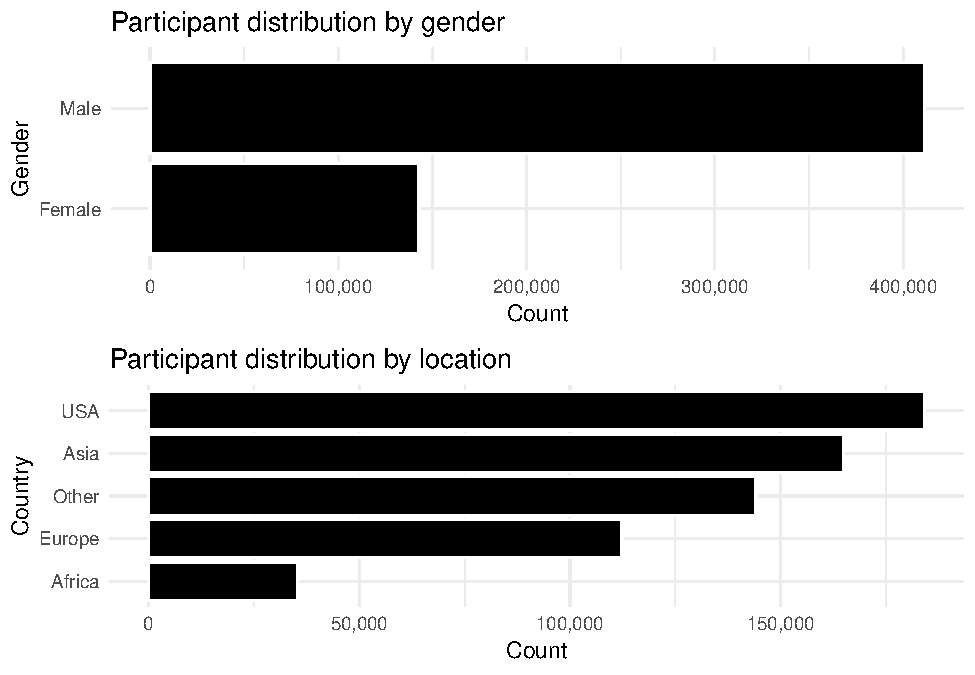
\includegraphics[width=1\linewidth]{initial-draft_files/figure-latex/unnamed-chunk-5-1} 

}

\caption{Descriptive statistics \label{descriptive_plots}}\label{fig:unnamed-chunk-5}
\end{figure}

As the descriptive statistics in Figure \ref{descriptive_plots}
indicate, majority of the participants are male. Also, USA and Asia
contribute most to the number of participants (note that we group
participants in the data set by continent).

To characterize initial drop-out on MOOCs, we define a participant as
`engaged' if they register and view at least one video from the course
(it follows that those who browsed more than one video and those who
earned certificates are also classified as `engaged'). Similarly, a
participant is classified as `not engaged' if they register but never
turn up, i.e., they drop-out even before starting the course. Figure
\ref{activity_status} summarizes the distribution of participants into
these two categories across the 16 courses.

\begin{figure}[p]

{\centering 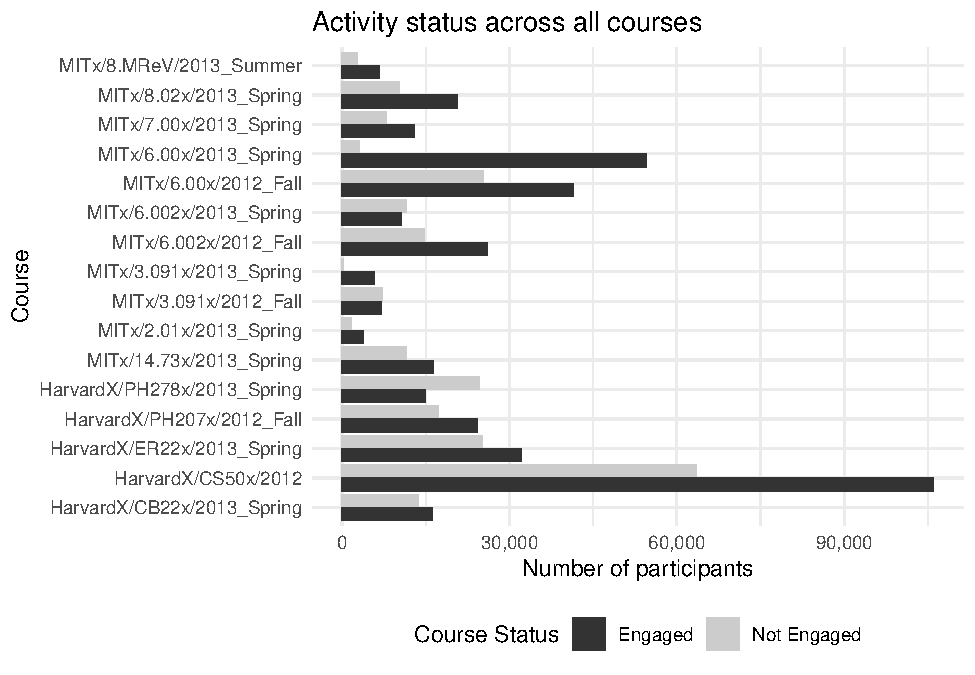
\includegraphics[width=1\linewidth,height=1\textheight]{initial-draft_files/figure-latex/unnamed-chunk-6-1} 

}

\caption{Activity Status \label{activity_status}}\label{fig:unnamed-chunk-6}
\end{figure}

Since our objective is to predict initial drop-out, our data is limited
to the behavior of participants before the course begins. We note that
this is in contrast to predictive models of grades or non-completion in
prior research, where significantly more data is available (e.g., number
of chapters accessed, number of videos, discussion forum activity).
While the lack of rich data poses challenges in model building, our
endeavor is to select a model that is most accurate in predicting
drop-out given the data.

\subsection{Predicting Initial
Dropout}\label{predicting-initial-dropout}

We note from Figure \ref{activity_status} that for every course, the
`not engaged' category presents a significant challenge. On an average,
the initial drop-out rate on the Harvard and MIT MOOCs is
\texttt{36.9\%}, which is disconcerting in the context of our earlier
discussion on public policy initiatives. Since there are no prior
studies on initial drop-out, the features used in our machine learning
algorithms are drawn from consumer research theory.

We conceptualize the MOOC participant as a consumer of course
information. The purchase (i.e., course registration) is done in advance
but the product (i.e., the course) is delivered at a later date. In the
context of initial dropout, we argue that there are three factors that
might lead early registrants to drop out before the course begins.
First, at the point of registration, participants are excited by the
content of the course and commit to begin the course. However, since the
course is delivered at a later stage, the tangible benefits from course
completion accrue only in the future. This is a key facet of the current
design of MOOCs and is closely related to theories of customer
impatience in the digital world. In this body of research the central
argument is that one a purchase is made, informed, fully visible and
on-time delivery process is the new norm (Daugherty, Bolumole, \& Grawe,
2018). Customers are willing to accept delayed outcomes only if a longer
waiting time results in a higher future value (Marino, Zotteri, \&
Montagna, 2018). Further, for lower-valued outcomes, time sensitivity
(i.e., the value placed on time) is higher (Thaler, 1981). Translating
these findings to the MOOC environment, we argue that while participants
are aware of the timelines of course delivery at the point of
registration, activity commences only close to the launch date of the
course. This lack of visible activity leads to an unresolved impatience.
The issue is exacerbated by the fact that growth spurts and attrition
that characterize the run-up to start of a course make community
formation difficult (Yang et al., 2013). The situation is especially
dire for participants whose motivation to join the MOOC is not
certification but fun or convenience (Belanger \& Thornton, 2013). For
these participants, the innate desire that drives them to register might
already be quenched by the act of registration. When the course starts
at a later stage, this event has much lesser utility. Following these
arguments, we operationalize the waiting time of participants as the
lead time between the date of registration of the participant and the
start date of the course. We expect that the date of registration, i.e.,
whether the participant registered early or late (relative to the course
start date) might be strongly predictive of initial dropout.

Second, a peculiar aspect of the data set is that the content of courses
within the data set is varied (for e.g., the courses include Ancient
Greek Hero and Introduction to Solid State Chemistry) and draws a wide
range of participants(Ho et al., 2014). Prior research indicates that
the completion rates on MOOCs are low across different course types
(Onah et al., 2014). In this research, we propose to validate this
finding in the case of initial drop-out as well. Consequently, we expect
the course content to have no effect on the willingness of the
participants to attend the course.

Third, we expect participant demographics to be reflective of the
infrastructure available in order to successfully engage with a MOOC.
For e.g., a participant from United States is expected to have access to
better internet facilities compared to a participant from Rwanda.

Following the descriptive measures and the arguments presented in this
section, we summarize our exploration of initial drop-out into the
following research questions:

\emph{RQ1: Early registration is strongly predictive of initial
drop-out}

\emph{RQ2: The subject of the course is not an important predictor of
initial drop-out}

\emph{RQ3: Demographics of a participant are strongly predictive of
initial drop-out}

\section{MODELING INITIAL DROPOUT}\label{modeling-initial-dropout}

In this section, we present predictive models for initial drop-out using
3 methods - Logistic Regression, Gradient Boosting and Neural Networks.

\subsection{Preprocessing}\label{preprocessing}

Engagement status was used as the label (coded 1 for `engaged' and 0 for
`not engaged) to be predicted in all our models. The features used to
predict the engagement status were extracted from age, gender, country
and date of registration. Following the discussion in section 2.3, we
added a new variable \texttt{joined\_early\_or\_late} by subtracting the
start date of a course from the date of registration by the participant.
We expect this variable to be the key predictor in our model (RQ1). The
other key variables included were age, gender and country (one-hot
encoded). Finally, we excluded the participants who registered for more
than one course (this allows us to justify the independent samples
assumption underlying the models). The final sample size on which the
models were evaluated is \(n = 316,917\).

\subsection{Model Execution}\label{model-execution}

Since we want our models to be strongly predictive of drop-out, we
attach prime importance to misclassified participants. In particular, we
want the number of participants who were misclassified as non drop-outs
to be minimum. To enforce this we scored our models using the AUC of the
ROC curve as the metric and selected the final model hyper parameters
based on 10-fold cross validation with 3 repeats. To account for the
class imbalance we observe in Figure \ref{descriptive_plots}, we follow
prior literature and employ the Synthetic Minority Over-sampling
Technique (SMOTE) to form the training set (chosen as 80\% of the entire
data set).

Logistic regression was executed using L2-regularization with the
regularization strength as the hyper parameter. For Gradient Boosting,
we use the \texttt{xgBoost} algorithm (Chen \& Guestrin, 2016), with
depth of the trees and the number of estimators tuned as hyper
parameters during training (we performed a random grid search over a
larger parameter space to arrive at a shortlist). The neural networks
were composed of a sequence of fully connected layers with the number of
units per layer and the number of layers tuned during training. The
final model comprised 9 fully connected layers, with 32 units in each
layer (total number of trainable parameters \(=4,417\)).

\subsection{Results}\label{results}

\begin{figure}[p]

{\centering 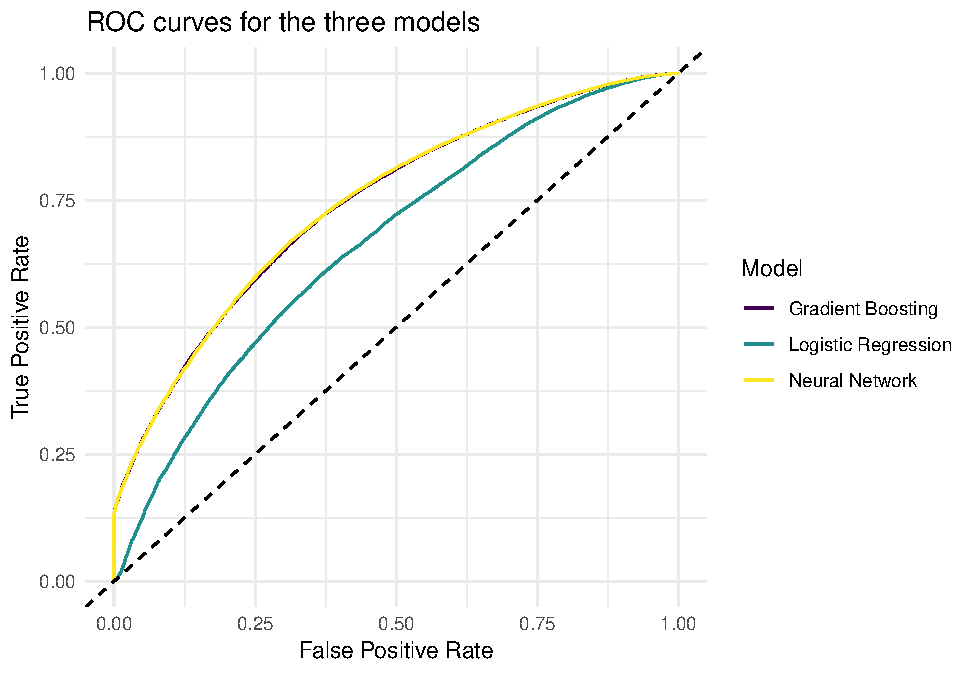
\includegraphics[width=1\linewidth]{initial-draft_files/figure-latex/unnamed-chunk-7-1} 

}

\caption{ROC curves for the 3 model fits \label{roc_curves}}\label{fig:unnamed-chunk-7}
\end{figure}

As can be inferred from \ref{roc_curves}, Gradient Boosting and Neural
Networks perform much better than Logistic Regression. However, since
the Gradient Boosting model had a higher accuracy on the test set
(76.1\%) we choose this as our final model.

\section{Discussion}\label{discussion}

The results presented in Section 3 indicate that the Gradient Boosted
Model is a good model for the data set. In order to address the research
questions posed in Section 2, we now move to probe the relative
importance of the factors in the predictive ability of the model on the
data set. Relative importance of a feature is computed by averaging
(across all trees) the number of times this feature is selected for the
split weighted by the improvement to the resulting model (Elith,
Leathwick, \& Hastie, 2008). Figure \ref{feature_importance} shows the
relative importance of the top 5 features that contribute most to the
predictive ability of the final Gradient Boosting Model on the test set.

\begin{figure}[p]

{\centering 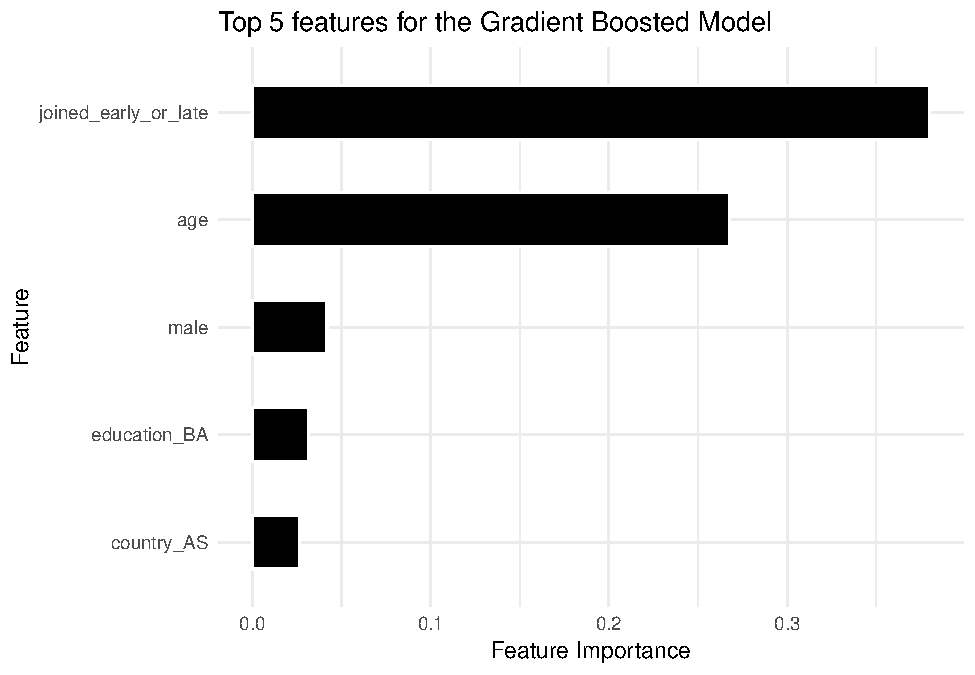
\includegraphics[width=1\linewidth]{initial-draft_files/figure-latex/unnamed-chunk-8-1} 

}

\caption{Feature importance plot of the Gradient Boosted Model \label{feature_importance}}\label{fig:unnamed-chunk-8}
\end{figure}

Figure \ref{feature_importance} indicates that the most important
feature to the prediction of initial drop-out is whether the participant
joined early (validating RQ1). Also, the course of study is not an
important predictor for initial drop-out validating RQ2. Further,
contrary to our expectation summarized in RQ3, our results indicate that
education and country are not on the same scale of importance as early
registration. This is surprising since we expect participants with
higher education levels to be more disciplined in attending and
completing MOOCs (given that they have attended and completed courses
within their formal education). The emergence of age as a stronger
predictor is a surprising finding we wish to explore in further
research.

In sum, we conclude that early registration is a key predictor of
initial dropout. This has important implications for the marketing and
execution of MOOCs. In practice, we observe that little attention is
paid to monitoring of participants before the course begins and our
results indicate that neglecting this phase has a devastating effect on
the dropout rate. Our results indicate that early registrants need to be
watched carefully and nudged to begin the course. We submit that this is
paramount for government initiatives, and we strongly advocate the
allocation of resources and attention to participants who have
registered early. Our results also indicate that the course of study is
not predictive of initial drop-out, and we propose that decision makers
do not make any distinction among courses while allocating resources. It
is important to note that while the precise initial dropout rates might
differ across courses, the subject of the course itself is not
predictive of initial dropout.

This study makes several important contributions to existing literature
on MOOCs. First, our conceptualization of a MOOC participant as a
consumer allows us to draw upon prior research on consumer behavior to
choose predictive features for our machine learning algorithms. We
submit that our approach to predictive modeling is novel in this aspect
- while our methods are rooted in data mining, the choice of predictive
features in these models is guided by consumer research. Second, our
results crystallize key factors that are predictive of initial drop-out
and can aid decision makers to market MOOCs effectively. Third, our
final model can be used to flag participants who are most likely to drop
out before the course begins. Our proposal is to utilize the predictions
from our model to fine tune marketing efforts directed at reduction in
the initial drop-out rate. All the code used for the modeling and data
processing is available in a \texttt{git} repository and can be
replicated by other scholar/practitioners to design MOOCs.

Since this study is one of the first to probe initial drop-out, it is
limited by the analysis of the secondary data. However, by using
powerful machine learning methods, we are able to crystallize key
features decision makers should be aware of while launching MOOCs. In
the next phase of research, we wish to undertake primary research to
understand the decision-making process of MOOC drop-outs and incorporate
the findings from this research into better predictive models of initial
dropout.

\newpage 

\section*{References}\label{references}
\addcontentsline{toc}{section}{References}

\hypertarget{refs}{}
\hypertarget{ref-bast2018swayam}{}
Bast, F. (2018). Learning on the go. \emph{The Hindu}. Retrieved from
\url{https://www.thehindu.com/education/learning-on-the-go/article24418318.ece}

\hypertarget{ref-belanger2013bioelectricity}{}
Belanger, Y., \& Thornton, J. (2013). Bioelectricity: A quantitative
approach duke university's first mooc.

\hypertarget{ref-chen2016xgboost}{}
Chen, T., \& Guestrin, C. (2016). Xgboost: A scalable tree boosting
system. In \emph{Proceedings of the 22nd acm sigkdd international
conference on knowledge discovery and data mining} (pp. 785--794). ACM.

\hypertarget{ref-daugherty2018impatience}{}
Daugherty, P. J., Bolumole, Y., \& Grawe, S. J. (2018). The new age of
customer impatience: An agenda for reawakening logistics customer
service research. \emph{International Journal of Physical Distribution
\& Logistics Management}.

\hypertarget{ref-elith2008working}{}
Elith, J., Leathwick, J. R., \& Hastie, T. (2008). A working guide to
boosted regression trees. \emph{Journal of Animal Ecology},
\emph{77}(4), 802--813.

\hypertarget{ref-ho2014harvardx}{}
Ho, A., Reich, J., Nesterko, S., Seaton, D., Mullaney, T., Waldo, J., \&
Chuang, I. (2014). HarvardX and mitx: The first year of open online
courses, fall 2012-summer 2013.

\hypertarget{ref-kizilcec2015attrition}{}
Kizilcec, R. F., \& Halawa, S. (2015). Attrition and achievement gaps in
online learning. In \emph{Proceedings of the second (2015) acm
conference on learning@ scale} (pp. 57--66). ACM.

\hypertarget{ref-kross2018students}{}
Kross, S., \& Guo, P. J. (2018). Students, systems, and interactions:
Synthesizing the first four years of learning@ scale and charting the
future. In \emph{Proceedings of the fifth annual acm conference on
learning at scale} (p. 2). ACM.

\hypertarget{ref-marino2018consumer}{}
Marino, G., Zotteri, G., \& Montagna, F. (2018). Consumer sensitivity to
delivery lead time: A furniture retail case. \emph{International Journal
of Physical Distribution \& Logistics Management}, \emph{48}(6),
610--629.

\hypertarget{ref-onah2014dropout}{}
Onah, D. F., Sinclair, J., \& Boyatt, R. (2014). Dropout rates of
massive open online courses: Behavioural patterns. \emph{EDULEARN14
Proceedings}, 5825--5834.

\hypertarget{ref-peters2018moocsevolved}{}
Peters, D. (2018). MOOCs are not dead, but evolving. \emph{University
Affairs}. Retrieved from
\url{https://www.universityaffairs.ca/news/news-article/moocs-not-dead-evolving/}

\hypertarget{ref-thaler1981some}{}
Thaler, R. (1981). Some empirical evidence on dynamic inconsistency.
\emph{Economics Letters}, \emph{8}(3), 201--207.

\hypertarget{ref-whitehill2017delving}{}
Whitehill, J., Mohan, K., Seaton, D., Rosen, Y., \& Tingley, D. (2017).
Delving deeper into mooc student dropout prediction. \emph{arXiv
Preprint arXiv:1702.06404}.

\hypertarget{ref-yang2013turn}{}
Yang, D., Sinha, T., Adamson, D., \& Rosé, C. P. (2013). Turn on, tune
in, drop out: Anticipating student dropouts in massive open online
courses. In \emph{Proceedings of the 2013 nips data-driven education
workshop} (Vol. 11, p. 14).


\end{document}
